\chapter{Medidas de dinamismo para roteamento dinâmico de veículos}
\label{ch:medidas}
% TODO Introduzir o que seriam medidas e a importância delas para as pesquisas 
% com relação a roteamento dinâmico de veículos

% TODO adicionar outros exemplos de medidas, explicando para que servem

% TODO explicar o porque dinamismo e urgência foram escolhidas

De acordo com o \textcite{michaelis_dinamico_2019}, dinâmico é algo que evolui
permanentemente, mutável, que admite movimento ou mudança.
Portanto, problemas de roteamento dinâmico de veículos são problemas que 
evoluem com o tempo e que se modificam com o a chegada de novas informações 
\cite{psaraftis_dynamic_2015}.

Muitos dos problemas de roteamento do dia-a-dia são problemas de natureza
dinâmica: entrega de encomendas, entrega de comida, serviços de emergência
(ex.: bombeiros), táxis e transporte por aplicativos. 
Entretanto, estes problemas apresentam diferenças em suas características 
dinâmicas. 

Analisando com atenção percebe-se que existem problemas em que o número de
pedidos agendados (não dinâmicos) é grande quando comparado com os demais
problemas, um exemplo disso é o problema de entrega de encomendas, muitas das
entregas são conhecidas \textit{a priori}, entretanto, algumas encomendas de
emergência podem aparecer durante o período de operação.
Em contrapartida, existem problemas em que todos os pedidos são dinâmicos e
devem ser atendidos com a maior rapidez possível, como por exemplo os serviços
de bombeiros.
Existem também os casos intermediários, em que pedidos podem surgir em forma de
agendamento antecipado ou dinamicamente entretanto não existe urgência para o
cumprimento destes.
A entrega de alimentos, por exemplo, é um problema deste tipo.

Percebendo que estas diferentes características nos problemas dinâmicos eram 
também associadas a diferenças nas qualidades das soluções encontradas,
muitos pesquisadores tentaram criar medidas de dinamismo de forma a 
possibilitar a classificação de problemas e auxiliar na escolha de métodos de 
solução.

A Seção~\ref{sec:medidas_revisao} dedica-se a relatar algumas das medidas de
dinamismo propostas na área de roteamento dinâmico de veículos,
além de relatar alguns dos usos práticos dessas medidas. 
Posteriormente, a Seção~\ref{sec:medidas_van_lon} apresenta a definição das
medidas de dinamismo e urgência propostas por \textcite{van_lon_measures_2016}.
No Capítulo~\ref{ch:analise} usa-se estas medidas para analisar
e comparar os conjuntos de instância de \textit{benchmark} expostos no 
Capítulo~\ref{ch:instancias}.








\section{Revisão bibliográfica}\label{sec:medidas_revisao}

Proposta primeiramente por \citeonline{lund_vehicle_1996}, o grau de dinamismo
de uma instância de qualquer VRP dinâmico representa a razão entre a quantidade
de pedidos dinâmicos, que se fazem conhecidos em um instante
$\arrivalTime_\request > 0$, e a quantidade total de pedidos da instância:
%
\begin{equation}
  \degreeOfDynamism = \frac{\numberOfRequests_{\text{d}}}{\numberOfRequests},
  \label{eq:degreeOfDynamism}
\end{equation}

\noindent em que $\degreeOfDynamism$ é o grau de dinamismo e 
$\numberOfRequests_{d}$ o número de pedidos dinâmicos

Essa classificação proporcionou uma base para o estudo das relações entre o 
grau de dinamismo, os tipos de métodos usados para a solução dos 
problemas e as características das soluções obtidas.
\citeonline{wong_dynamic_2014}, por exemplo, mostram que existe uma relação não
linear entre o grau de dinamismo e o custo de transporte de uma instância de um
problema responsivo à demanda.
Suas análises numéricas elucidam a existência de um pico de ineficiência para
vários algoritimos heurísticos quando $\degreeOfDynamism \approx 0{,}7$, o que
os autores classificaram como ``zona de dilema''.
Através dessa descoberta \citeonline{wong_dynamic_2014} descrevem uma série de
políticas para que operadores de sistemas de transporte responsivos à demanda
(DRT - \textit{Dynamic Responsive Transpot}) possam seguir para permanecer 
longe da ``zona de dilema''.

Similarmente, \citeonline{larsen_partially_2002} usam essa mesma medida de 
grau de dinamismo para estudar a relação entre o custo de rota para o 
problema parcialmente dinâmico do reparador itinerante 
(PDTRP - \textit{Partially Dynamic Traveling Repairman Problem}).
Os resultados empíricos ilustram uma relação linear entre o nível de
dinamismo de uma instância e o custo da rota de um sistema relativamente ativo.

Posteriormente, baseando-se no fato de que o instante de chegada dos pedidos
dinâmicos também deve afetar o grau de dinamismo,
\textcite{larsen_dynamic_2000} define o grau efetivo de dinamismo por:
%
\begin{equation}
  \eDegreeOfDynamism = 
  \frac{1}{\numberOfRequests}
  \sum_{\request \in \requests}
  {
    \frac{\arrivalTime_\request}{\planingHorizon}
  },
  \label{eq:eDegreeOfDynamism}
\end{equation}

\noindent em que $\eDegreeOfDynamism$ é o grau efetivo de dinamismo e 
representa a média da razão entre os instantes que os pedidos são conhecidos 
quando comparados com o último instante possível para a chegada deles, 
$\planingHorizon$, no caso. Os instantes de chegada dos pedidos estáticos são 
considerados igual a zero.

É importante destacar que apesar de representarem formas de cálculo diferentes,
o grau de dinamismo e o grau de dinamismo efetivo compartilham entre si o mesmo
intervalo de possíveis valores, contido entre $0$ e $1$, sendo que
$\degreeOfDynamism = \eDegreeOfDynamism = 0$ classifica uma instância
totalmente estática e $\degreeOfDynamism = \eDegreeOfDynamism = 1$ representa
uma totalmente dinâmica.

Em um outro estudo, \citeonline{larsen_classification_2007} usam o grau efetivo
de dinamismo para classificar os problemas de roteamento dinâmico de veículos
(DVRP - \textit{Dynamic Vehicle Routing Problem}) em três classes distintas:
fracamente, moderadamente e fortemente dinâmicos, cujos intervalos de valores 
$\eDegreeOfDynamism$ correspondem, respectivamente, a $\eDegreeOfDynamism \leq
0{,}3$, $0{,}3  < \eDegreeOfDynamism < 0{,}8$ e $0{,}8 \leq
\eDegreeOfDynamism$.
A intenção dessa segregação de problemas é facilitar a escolha de um algoritmo
para a sua solução.

\citeonline{larsen_dynamic_2000} também estende o grau de dinamismo efetivo
para problemas com janelas de tempo.
A ideia é contabilizar também o nível de urgência de cada um dos pedidos, 
sendo que o nível de urgência é visto como o tempo de reação disponível
para que o sistema, após receber a informação do pedido no instante
$\arrivalTime_\request$, possa passar pelo nó de coleta $\originNode$
antes do limite superior da janela de tempo de coleta
$\latestTimeWindow_{\originIndex}$.
\citeonline{larsen_dynamic_2000} define que: 
%
\begin{equation}
  \reactionTime_\request = \latestTimeWindow_{\originIndex}
                           - \arrivalTime_\request,
\end{equation}

\noindent em que $\reactionTime_\request$ é o tempo de reação do pedido
$\request$.

Com isso, o grau efetivo de dinamismo, quando contabilizado o tempo de reação,
é definido por \cite{larsen_dynamic_2000}:
%
% TODO tentar alinhar os sinais de igualdade das duas equações a seguir
%
\begin{equation}
  \eDegreeOfDynamismTW = 
  \frac{1}{\numberOfRequests}
  \sum_{\request \in \requests}
  {
    \left(
    \frac{\planingHorizon - (\latestTimeWindow_\originIndex
                             - \arrivalTime_\request)}
         {\planingHorizon}
    \right),
  }
\end{equation}

\begin{equation}
  \eDegreeOfDynamismTW = 
  \frac{1}{\numberOfRequests}
  \sum_{\request \in \requests}
  {
    \left(
      1 - \frac{\reactionTime_\request}{\planingHorizon}
    \right),
  }
\end{equation}

\noindent em que $\eDegreeOfDynamismTW$ é o grau efetivo de dinamismo com 
janelas de tempo.

É importante destacar que, assim como as medidas apresentadas anteriormente, o
grau efetivo de dinamismo com janelas de tempo também apresenta valores somente
dentro do intervalo $[0, 1]$.

\citeonline{pillac_review_2013} relata que todas as três medidas expostas neste
capítulo se provaram úteis para capturar os aspectos do dinamismo relacionados
com o tempo.
Entretanto essas medidas não levam em consideração outras fontes de dinamismo,
como a distribuição espacial dos pedidos e o tempo de viagem entre pedidos.
Essas fontes de dinamismo se mostram bastante importantes quando o objetivo é
minimizar o tempo de resposta do sistema.

Além disso, apesar de não considerada na definição das medidas de dinamismo, a
frequência com que os pedidos chegam ao sistema tem um grande impacto no tempo
disponível para otimização \cite{pillac_review_2013}.
Similarmente, \citeonline{kilby_dynamic_1998} fazem a observação de que a
frequência dos pedidos influencia a quantidade de vezes que o algoritmo
precisa ser executado.
Eles destacam que instâncias em que os pedidos estão agrupados em
pequenos intervalos de tempo geram menos necessidade de mais rodadas de
otimização do que casos onde os pedidos estão separados um dos outros de 
maneira uniforme.

No final do seu artigo, \citeonline{larsen_classification_2007} recomendam
para futuras pesquisas a extensão do grau de dinamismo para que ele também 
leve em conta outras características do problema, como o tamanho dos tempos de 
serviço e o carregamento dos pedidos.
Eles também mencionam que é desafiador encontrar uma medida única com
capacidade de apreender múltiplas características de uma instância.






\section{Medida de dinamismo e urgência proposta por Van Lon, Ferrante et al.
         (2016)}\label{sec:medidas_van_lon}
Com o intuito de produzir medidas que melhor representam as características
relacionadas ao dinamismo de um DPDPTW, \citeonline{van_lon_measures_2016} 
propõem uma nova definição para a medida de dinamismo, como também uma nova
medida denominada urgência.
Apesar do foco ser em problemas DPDPTW, \citeonline{van_lon_measures_2016}
afirmam que os conceitos de dinamismo e urgência não são limitados a este tipo
de problema, podendo ser usados em qualquer DVRP.

Como premissa, os autores consideram que estes parâmetros devem ser 
relacionados apenas ao problema, e portanto, o algoritmo usado para solução 
não deve influenciar em seus valores.
Entretanto, é desejado que essas medidas colaborarem para a classificação das 
instâncias e assim permitam a análise da eficácia dos algoritmos quando 
submetidos a diferentes condições de dinamismo e urgência. 
Além disso, \citeonline{van_lon_measures_2016} afirmam que as medidas devem ser 
interdependentes, não podendo haver correlação entre suas definições. 

O restante desse capítulo apresenta a definição, feita por
\citeonline{van_lon_measures_2016}, das duas medidas usadas para a determinação
das características temporais dos pedidos de uma instância de um problema de 
roteamento dinâmico qualquer.






\subsection{Dinamismo}\label{sec:dinamismo}
Define-se, primeiramente, que o grau de dinamismo é dado através da 
continuidade de mudança das informações presentes para um sistema. 
Por esse ponto de vista, todo evento que introduz informações novas para o 
problema, como a chegada de um pedido, a quebra de um veículo ou o cancelamento
de uma viagem, é classificado como uma mudança.
Um cenário muito dinâmico é caracterizado por mudanças contínuas, em oposição a
um cenário pouco dinâmico, onde mudanças ocorrem ocasionalmente.
A Figura~\ref{fig:van_lon_measures_2016_dynamism} demonstra, 
através de exemplos, as diferentes formas de distribuição de mudanças,
associando cada uma à um grau de dinamismo.

% TODO: mudar para arquivo .eps
\begin{figure}[H]
    \begin{center}
        \makebox[\textwidth]
          {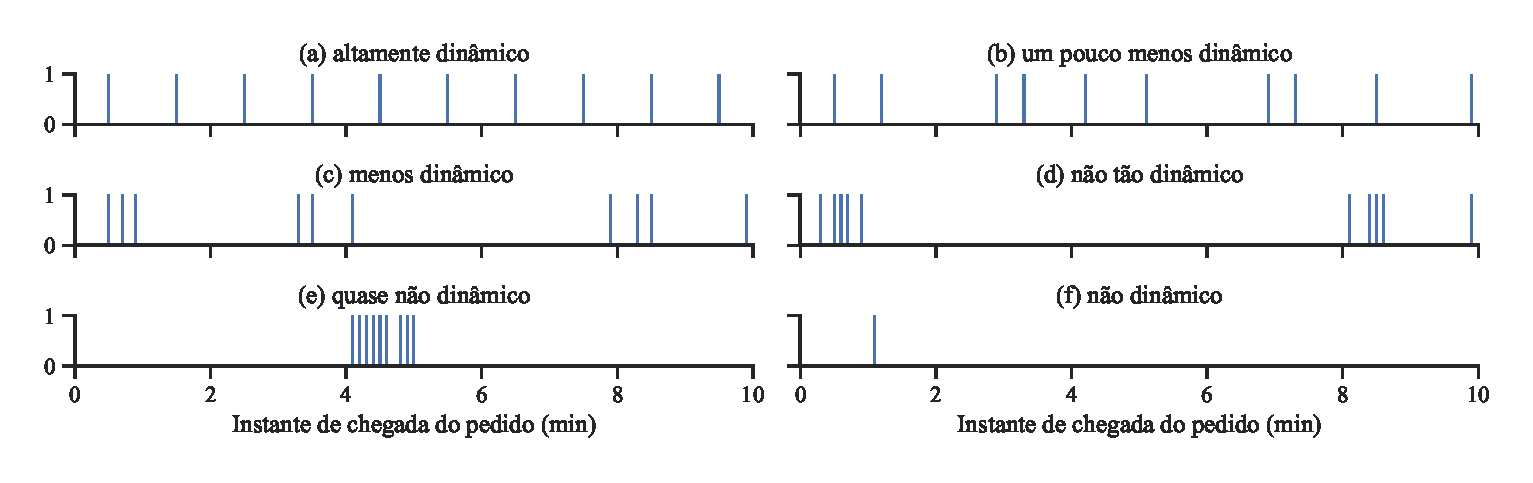
\includegraphics[width=\textwidth]{./fig/dynamism_sample.eps}}
        \caption{Exemplos de cenários com diferentes valores de dinamismo 
        \cite{van_lon_measures_2016}}
        \label{fig:van_lon_measures_2016_dynamism}
    \end{center} 
\end{figure}

Todos os gráficos da Figura~\ref{fig:van_lon_measures_2016_dynamism},
identificados pelas letras (a-f), representam um cenário com horizonte de 
planejamento de 10 minutos e com um total de 10 pedidos dinâmicos.
No cenário da Figura~\ref{fig:van_lon_measures_2016_dynamism}(a) os eventos 
acontecem em intervalos igualmente espaçados e distribuídos proporcionalmente 
no horizonte de planejamento.
Nos cenários da Figura~\ref{fig:van_lon_measures_2016_dynamism}(b, c) 
pode-se ver que mudanças ocorrem de maneira menos distribuída, apresentando uma
leve concentração de pedidos.
Na Figura~\ref{fig:van_lon_measures_2016_dynamism}(d, e) todos os eventos
ocorrem em uma ou duas bateladas, diminuindo ainda mais a distribuição dos
pedidos e, com isso, diminuindo o dinamismo dos cenários.
Na Figura~\ref{fig:van_lon_measures_2016_dynamism}(f) todos os eventos chegam
em um mesmo instante, resultando em um cenário sem dinamismo
\cite{van_lon_measures_2016}.

Para formular a medida de dinamismo \citeonline{van_lon_measures_2016} definem
primeiramente uma lista, $\intervalsBetweenArrivals$, de intervalos de chegadas
entre pedidos:
%
\begin{equation}
    \intervalsBetweenArrivals = 
    \{\intervalBetweenArrivals_0,\intervalBetweenArrivals_1,\ldots, 
    \intervalBetweenArrivals_{\numberOfRequests-2}\} = 
    \{\arrivalTime_j - \arrivalTime_i 
    \mid j = i + 1 \wedge \forall i, j \in \pickupNodes\},
    \label{eq:van_lon_measures_2016_intervalsBetweenArrivals}
\end{equation}
%
\begin{equation}
    |\intervalsBetweenArrivals| = \numberOfRequests - 1.
    \label{eq:van_lon_measures_2016_intervalsBetweenArrivalsSize}
\end{equation}

\noindent em que $\intervalsBetweenArrivals$ é a lista de intervalos entre 
chegada de pedidos e $\intervalBetweenArrivals_\request$ o intervalo de tempo 
entre a chegada do pedido $\request$ e seu sucessor. 
Portanto, $\intervalsBetweenArrivals$ representa uma lista com todos os valores
de intervalos de tempo em que o estado do sistema não é alterado, ordenados
cronologicamente.
Essa lista possui uma quantidade de valores $|\intervalsBetweenArrivals|$ 
cuja definição é (\ref{eq:van_lon_measures_2016_intervalsBetweenArrivalsSize}).

Para fins de comparação, é definido um intervalo de chegada perfeito,
$\perfectInterval$. Este é dado por:
%
\begin{equation}
    \perfectInterval = \frac{H}{\numberOfRequests},
    \label{eq:van_lon_measures_2016_perfectInterval}
  \end{equation}

\noindent em que $\perfectInterval$ é o intervalo de chegada perfeito.

Com isso obtêm-se o espaço de tempo entre pedidos do cenário com maior
dinamismo possível, dada uma quantia de pedidos $\numberOfRequests$ 
e um horizonte de planejamento $\planingHorizon$.
Voltando ao exemplo da Figura~\ref{fig:van_lon_measures_2016_dynamism},
temos que o cenário (a) seria o cenário em que
$\intervalBetweenArrivals_\request = \perfectInterval, \forall
\intervalBetweenArrivals_\request \in \intervalsBetweenArrivals$.
Ou seja, dos cenários apresentados na 
Figura~\ref{fig:van_lon_measures_2016_dynamism}, o cenário (a) é, além do mais
dinâmico dos cenários da figura, também o cenário mais dinâmico possível pra
esses valores de $\numberOfRequests$ e $\planingHorizon$.

Tendo os conceitos de intervalos entre chegadas de pedido e o intervalo de
chegada perfeito definidos, pode-se definir o desvio,
$\deviationFromPerfectInterval$, entre os intervalos de chegada contidos em
$\intervalsBetweenArrivals$ com o intervalo de chegada perfeito,
$\perfectInterval$:
%
\begin{equation}
    \deviationFromPerfectInterval_i =
        \begin{cases}
            \perfectInterval - \intervalBetweenArrivals_i,
            & \text{se $i = 0$ 
                    e $\intervalBetweenArrivals_i < \perfectInterval$} \\
            \perfectInterval - \intervalBetweenArrivals_i 
            + \frac{\perfectInterval-\intervalBetweenArrivals_i}
                   {\perfectInterval}
            \cdot \deviationFromPerfectInterval_{i-1},
            & \text{se $i > 0$ 
                    e $\intervalBetweenArrivals_i < \perfectInterval$} \\
            0, & \text{caso contrário},
        \end{cases}
    \label{eq:van_lon_measures_2016_deviationFromPerfectInterval}
\end{equation}

\noindent em que $\deviationFromPerfectInterval_i$ é o desvio 
entre os intervalos de chegada $\intervalBetweenArrivals_i$ e o 
$\perfectInterval$. 
O termo ($\frac{\perfectInterval-\intervalBetweenArrivals_i}
{\perfectInterval} \cdot \deviationFromPerfectInterval_{i-1}$) serve para 
penalizar, de forma recursiva, a aglutinação de eventos em pequenos 
períodos de tempo.

% TODO: explicar melhor o que significa cada um dos casos da equação acima,
% assim como o conceito completo expresso por ela.

Consequentemente, o desvio total do cenário pode ser calculado por:
%
\begin{equation}
    \deviation = 
    \sum_{i=0}^{|\intervalsBetweenArrivals|} \deviationFromPerfectInterval_i.
    \label{eq:van_lon_measures_2016_totalDeviationFromPerfectInterval}
\end{equation}

Entretanto, faz-se necessária a normalização do desvio total do cenário com
relação ao desvio máximo possível.
Para isso, calcula-se o maior valor:
%
\begin{equation}
    \maxDeviation =
    \sum_{i=0}^{|\intervalsBetweenArrivals|} 
		\overline{\deviationFromPerfectInterval}_i,
    \label{eq:van_lon_measures_2016_bigestTotalDeviationFromPerfectInterval}
\end{equation}

\noindent em que:
%
\begin{equation}
    \overline{\deviationFromPerfectInterval}_i = \perfectInterval + 
        \begin{cases}
            \frac{\perfectInterval - \intervalBetweenArrivals_i}
								 {\perfectInterval} 
						\cdot \deviationFromPerfectInterval_{i-1},
						& \text{se $i>0$ e $\intervalBetweenArrivals_i 
                    < \perfectInterval$}\\
            0, & \text{caso contrário.}
        \end{cases}
    \label{eq:van_lon_measures_2016_bigestDeviationFromPerfectInterval}    
\end{equation}

Combinando  
(\ref{eq:van_lon_measures_2016_bigestTotalDeviationFromPerfectInterval})
e~(\ref{eq:van_lon_measures_2016_bigestDeviationFromPerfectInterval}), define-se 
dinamismo como:

\begin{equation}
      \dynamism = 1 - \frac{\deviation}{\maxDeviation} = 1 -
      \frac{\sum_{i=0}^{|\intervalsBetweenArrivals|}
			\deviationFromPerfectInterval_i}{\sum_{i=0}^{|\intervalsBetweenArrivals|}
      \overline{\deviationFromPerfectInterval}_i}.
      \label{eq:van_lon_measures_2016_dynamism}
\end{equation}

% TODO: Escrever interpretação das 4 equações anteriores






\subsection{Urgência}\label{sec:urgencia}

No contexto dos DVRPs, a urgência representa o tempo de reação disponível ao 
sistema de transporte para que ele consiga atender a um pedido.
Essa medida pode ser expressa através de unidades de tempo e definida pela 
diferença entre o instante de chegada de um pedido ($\arrivalTime_\request$) 
e o limite superior da janela de tempo de coleta 
($\latestTimeWindow_\originIndex$).
A Figura~\ref{fig:van_lon_measures_2016_urgency} exemplifica dois casos.

%TODO: converter imagem de png para eps
\begin{figure}[H]
    \begin{center}
        \makebox[\textwidth]{
          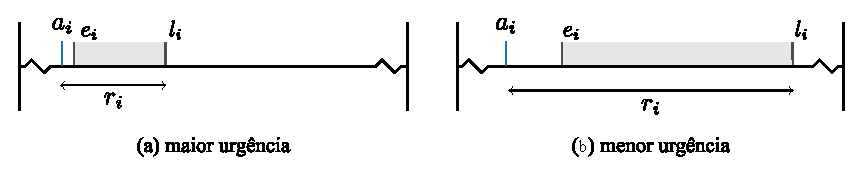
\includegraphics[width=\textwidth]{fig/urgency_sample.eps}}
        \caption{Exemplos de pedidos com diferentes valores de urgência 
                 \cite{van_lon_measures_2016}}
        \label{fig:van_lon_measures_2016_urgency}
    \end{center} 
\end{figure}

No cenário da Figura~\ref{fig:van_lon_measures_2016_urgency}(a) temos o exemplo
de um pedido com grande urgência, ou seja, menor tempo de reação.
Já no caso da Figura~\ref{fig:van_lon_measures_2016_urgency}(b) o tempo de 
reação é maior, portanto o pedido é menos urgente.

Baseando-se na Figura~\ref{fig:van_lon_measures_2016_urgency}, 
\citeonline{van_lon_measures_2016} define urgência por:
%
\begin{equation}
    \urgency_\request = 
    \reactionTime_\request =
    \latestTimeWindow_\request - \arrivalTime_\request,
    \label{eq:van_lon_measures_2016_urgency}
\end{equation}

\noindent em que $\urgency_\request$ é a urgência do pedido $\request$.

Para obter uma indicação da urgência de um cenário completo, pode-se computar a
média e o desvio padrão das urgências. 
Esta definição é similar ao grau de dinamismo efetivo com janelas de tempo 
proposto por \citeonline{larsen_dynamic_2000} e definido por
(\ref{eq:degreeOfDynamism})~e~(\ref{eq:eDegreeOfDynamism}).
Entretanto, existe uma diferença entre estas duas definições.
\citeonline{larsen_dynamic_2000} normaliza os valores do grau de dinamismo
efetivo com janelas de tempo usando o horizonte de planejamento.  
Já \citeonline{van_lon_measures_2016} acredita que a extensão do cenário e
a urgência devem ser independentes.


